\newpage
\section{Método da seção crítica}\label{sec:secao_critica}

O $C_{L\mathrm{max}}$ de asa limpa em baixa velocidade foi determinado pelo
método da seção crítica em $M = 0{,}2$, com a incidência de empenagem de
cruzeiro da seção anterior. Para cada posição de CG, com e sem a restrição
de trimagem, o ângulo de ataque foi aumentado até a distribuição de
coeficiente de sustentação local da asa, no plano normal ao enflechamento
(\texttt{cl\_norm} do AVL), alcançar o limite de $c_{\ell\mathrm{max}}$ dos
perfis otimizados. O limite usado é o do Lab 03 no plano normal, com a
correção da calibração do XFoil: 1,774 na raiz, 1,799 no meio e 1,734 na
ponta, interpolado linearmente entre as estações. Como o método é linear, o
cruzamento foi resolvido por interpolação na varredura de $\alpha$.

Uma primeira aplicação do método na asa sem torção revelou estol começando
na ponta, em $\eta = 0{,}89$, sobre a região do aileron, com
$C_{L\mathrm{max}}$ entre 0,83 e 0,92. Esse diagnóstico motivou a
otimização de torção apresentada na Seção 6, e os resultados a seguir
referem-se à asa final, já com a torção aplicada.

\begin{table}[H]
\centering
\caption{Resultados do método da seção crítica para os quatro casos, asa final.}\label{tab:secao_critica}
\renewcommand{\arraystretch}{1.25}
\begin{tabular}{lccc}
\toprule
Caso & $\alpha_{\mathrm{max}}$ [graus] & $C_{L\mathrm{max}}$ & $\delta_e$ [graus] \\
\midrule
CG dianteiro sem trimagem & 14,72 & 1,130 & 0,0 \\
CG dianteiro com trimagem & 14,77 & 1,036 & $-17{,}07$ \\
CG traseiro sem trimagem & 14,70 & 1,155 & 0,0 \\
CG traseiro com trimagem & 14,73 & 1,097 & $-10{,}70$ \\
\bottomrule
\end{tabular}
\end{table}

\begin{figure}[H]
\centering
\caption{Distribuições de coeficiente de sustentação da asa na condição de
estol, com a curva limite de $c_{\ell\mathrm{max}}$ dos perfis. A estrela
marca a seção crítica.}\label{fig:clxy}
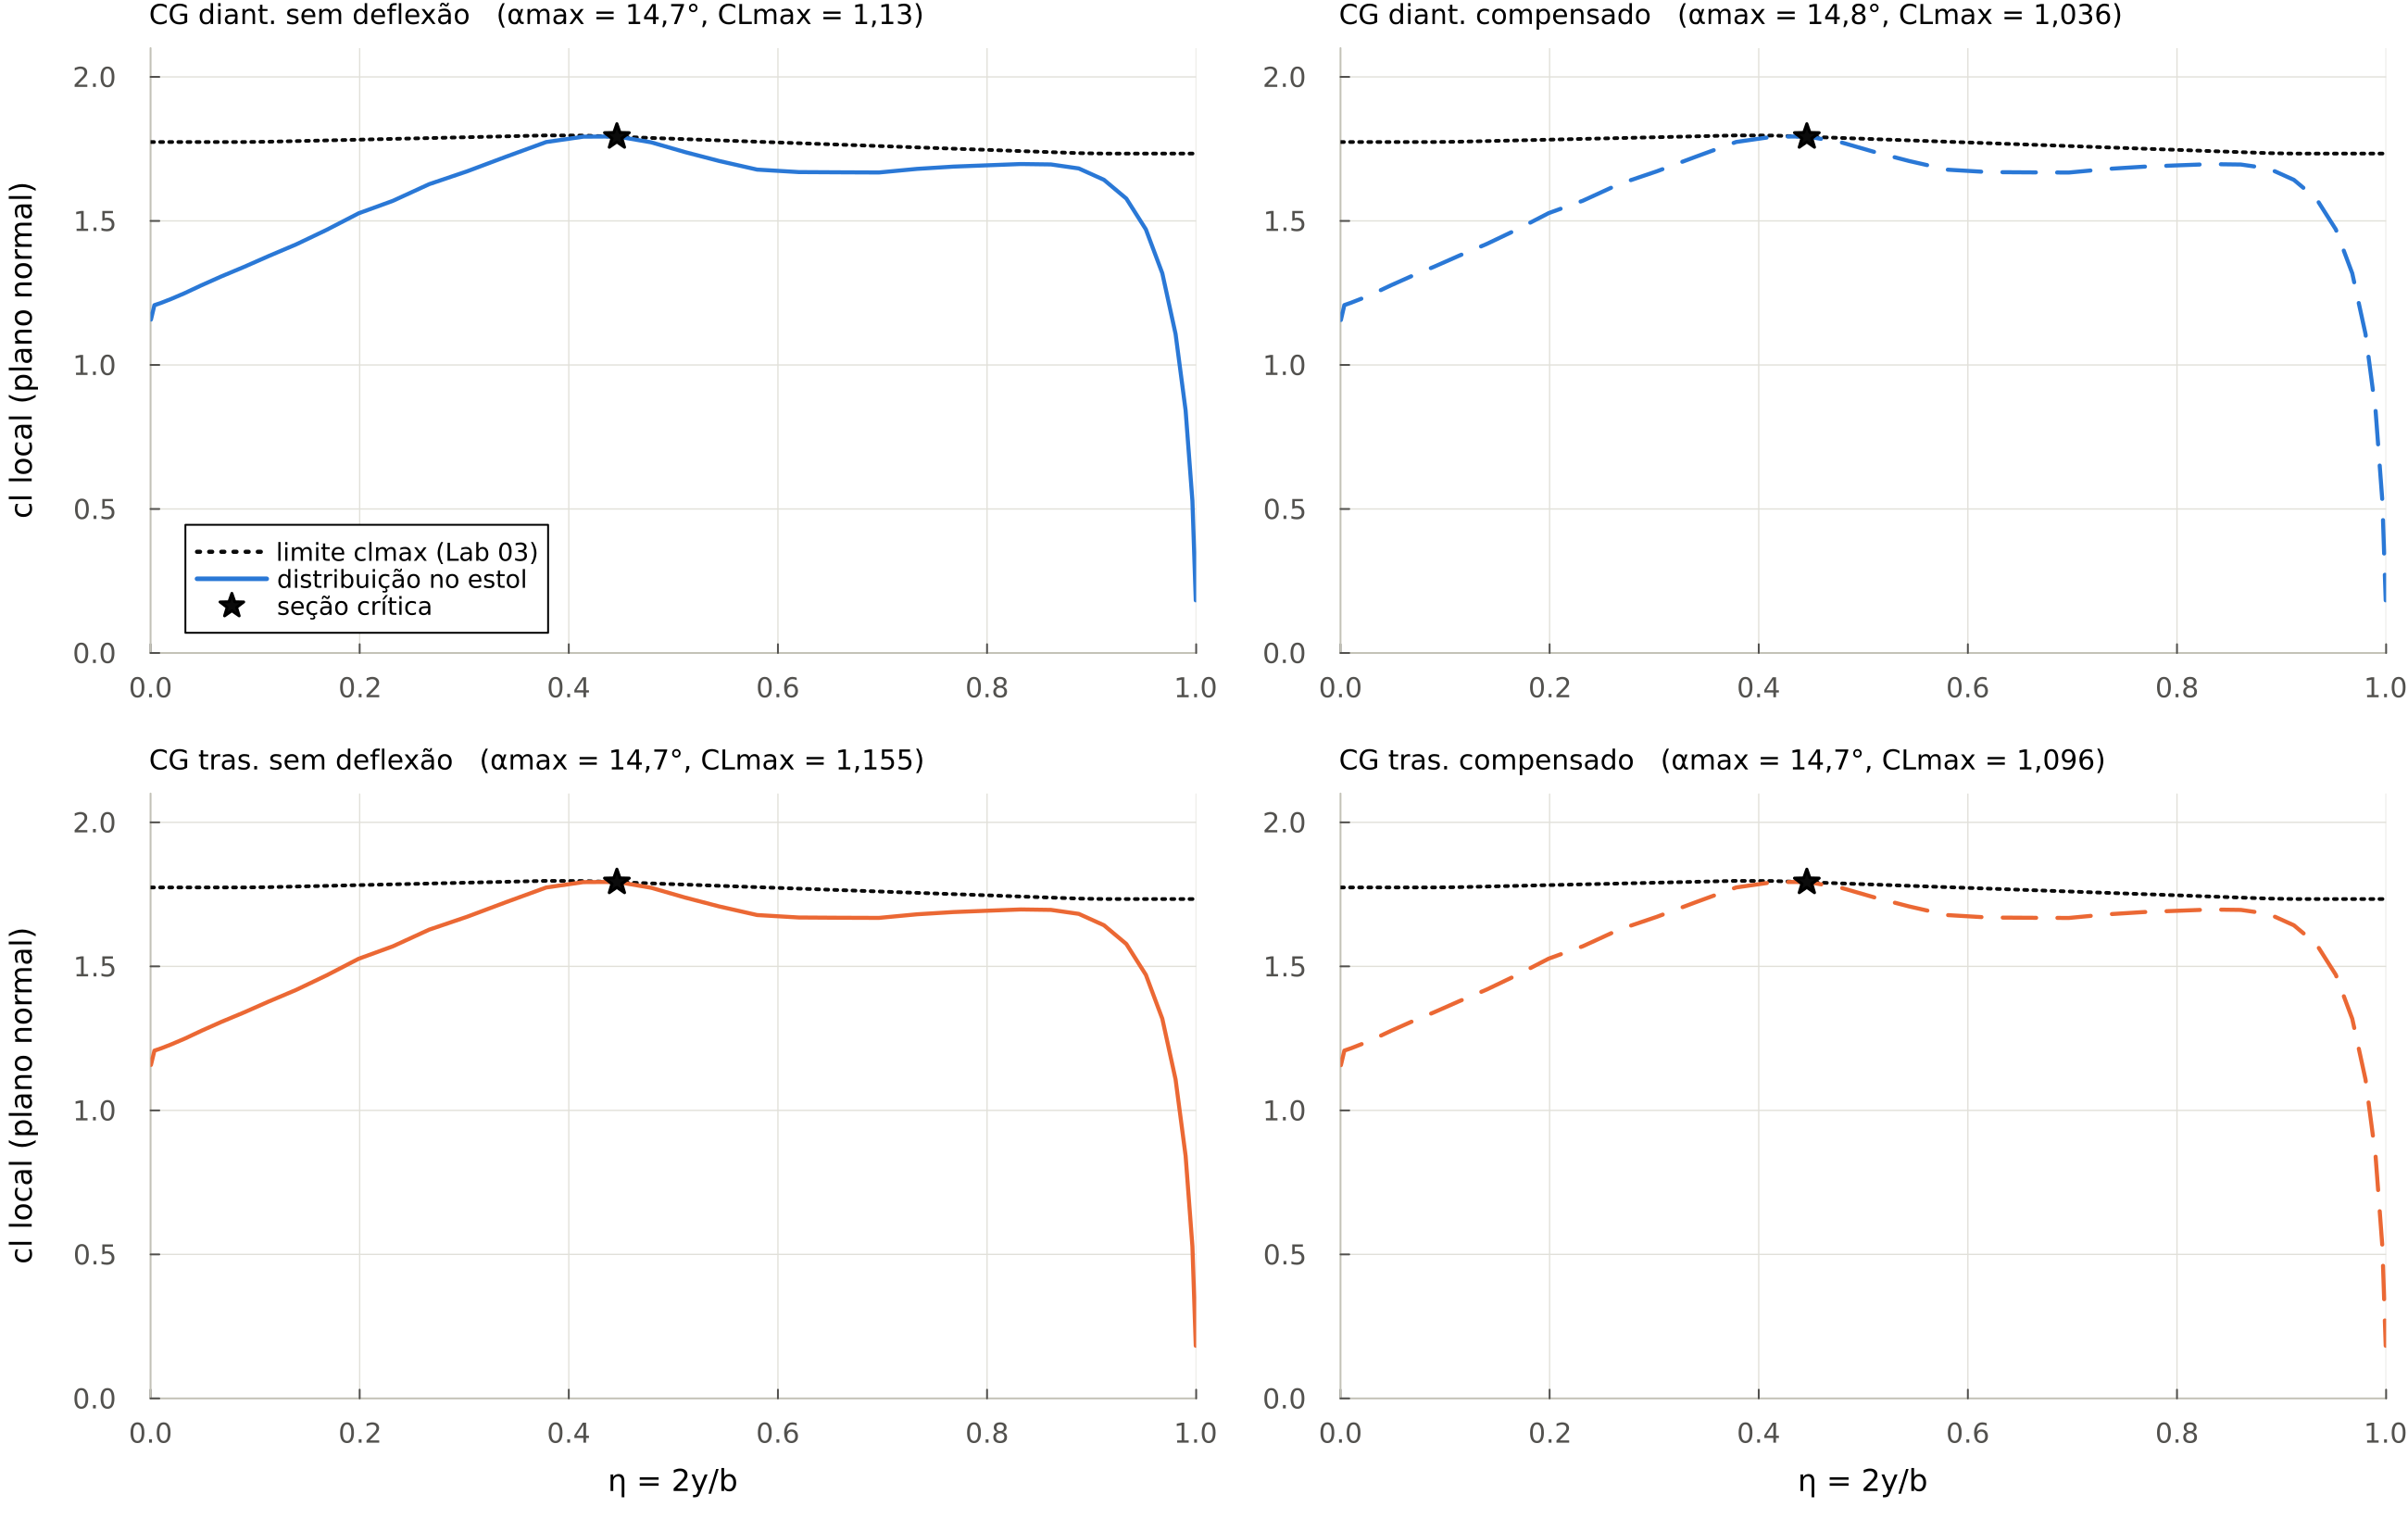
\includegraphics[width=\linewidth]{images/05_secao_critica/clxy_estol.png}
\end{figure}

O ângulo de estol é praticamente o mesmo nos quatro casos, em torno de
$14{,}7^\circ$, porque a distribuição de sustentação da asa quase não muda
com o CG ou com a trimagem. O que muda é o $C_{L\mathrm{max}}$ da
aeronave: a compensação exige força para baixo na empenagem, que subtrai
sustentação total, e o efeito é maior no CG dianteiro, onde o braço de
compensação é maior. O caso mais restritivo é o CG dianteiro com trimagem,
com $C_{L\mathrm{max}} = 1{,}036$.

\subsection*{Características de estol}

Com a torção otimizada, a seção crítica fica em $\eta = 0{,}45$ em todos
os casos: o estol começa na metade interna da asa, antes do aileron, que
ocupa de $\eta = 0{,}56$ a $\eta = 0{,}90$. A característica é adequada: a
separação inicial ocorre longe das superfícies de comando lateral e a
região da ponta mantém folga de sustentação, preservando o controle de
rolamento no início do estol.

Os valores de $C_{L\mathrm{max}}$, entre 1,04 e 1,16, ficam abaixo da
estimativa de asa limpa do \texttt{designTool}, de 1,33. Contribuem para a
diferença o limite de $c_{\ell\mathrm{max}}$ ser aplicado no plano normal,
o que equivale a um limite na direção da corrente cerca de 28\% menor, e o
desconto da força de compensação da empenagem, efeitos que a correlação
histórica do \texttt{designTool} não captura. A deflexão de profundor no
estol trimado do CG dianteiro, de $-17{,}1^\circ$, é alta mas permanece
dentro de batentes típicos de $\pm 25^\circ$.
